%%%%%%%%%%%%%%%%%%%%%%%%%%%%%%%%%%%%%%%%%%%%%%%%%%%%%%%%%%%%%%%%%%%%%%%%%%%
%%%                         O MODELO                                    %%%
%%%%%%%%%%%%%%%%%%%%%%%%%%%%%%%%%%%%%%%%%%%%%%%%%%%%%%%%%%%%%%%%%%%%%%%%%%%

\chapter{Descrição do Projeto}

% objetivos, ponto de partida, produtos e resultados esperados, tecnologias a serem usadas.
% + estrutura da solução nas fases de treinamento e aplicação

% ### METODOLOGIA ###

% ### Falar das seguintes ferramentas:
%   - DSR ok
%   - Trello
%   - Github

A seguir, serão apresentadas a metodologia e os softwares utilizados neste estudo, bem como as etapas detalhadas de sua implementação.

% Metodologia
\section{Metodologia}~\label{sec:metodologia}
Um ponto importante para a obtenção dos objetivos deste trabalho está relacionado a definição da metodologia que servirá como alicerce. Com a proposta de desenvolver e validar um método de análise da evolução molecular de vírus com base no uso de códons, a metodologia escolhida para isso foi o \gls{dsr}. Ela, proporcionou um framework teórico e prático para a criação de artefatos inovadores, como métodos, modelos ou frameworks, visando resolver problemas específicos~\cite{peffers_dsr_2007}. Neste projeto, a ferramenta de análise de genes virais baseada em códons é o produto que será desenvolvido e avaliado. Além disso, o \gls{dsr} enfatiza a validação e a avaliação da utilidade e eficácia do artefato em relação aos seus objetivos práticos. No caso deste projeto, a validação será realizada através da comparação dos resultados obtidos com a ferramenta proposta em relação às técnicas clássicas filogenéticas, que são amplamente utilizadas para a análise de genes virais. Essa comparação permitirá avaliar a eficácia e o valor agregado da abordagem baseada em códons.

Para a obtenção de sucesso ao utilizar o \gls{dsr} os seguintes passos serão seguidos:
\begin{enumerate}
  \item \textbf{Identificação do problema e definição dos objetivos:} Nesta fase, o problema a ser resolvido é identificado e compreendido em detalhes. No contexto deste projeto, isso envolveria a compreensão das limitações das abordagens existentes para a classificação de genes virais.
  \item \textbf{Concepção e planejamento:} Aqui, são definidos os objetivos do artefato a ser criado, suas características e funcionalidades. No projeto em questão, isso envolveria a definição da funcionalidade da ferramenta de análise de genes virais com base em códons.
  \item \textbf{Desenvolvimento dos artefatos:} Nesta etapa, os produtos desenvolvidos foram: todos os \textit{scripts}; \textit{datasets}; modelos e as ferramentas criadas.
  \item \textbf{Avaliação do artefato:} O artefato é testado e avaliado quanto à sua eficácia na resolução do problema. Isso pode incluir testes de desempenho, experimentos e comparações com métodos existentes.
  \item \textbf{Apresentar contribuições científicas:} Todos os resultados e contribuições obtidos serão disponibilizados de forma completa e detalhada na plataforma da \gls{uneb} e no repositório do projeto no GitHub do \gls{g2bc}~\footnote{Url do repositório: \url{https://github.com/G2BC/agua}}.
  \item \textbf{Iteração:} O processo é iterado conforme necessário. À medida que novos problemas ou insights surgem, os artefatos são aprimorados.
\end{enumerate}

Sendo assim, como apresentado na figura\ref{fig:processoDSR}, os passos citados anteriormente são realizados em uma iteração constante, até a obtenção do objetivo final.

\begin{figure}[htb]
  \centering
  \caption{Processo iterativo da metodologia \gls{dsr}.}
  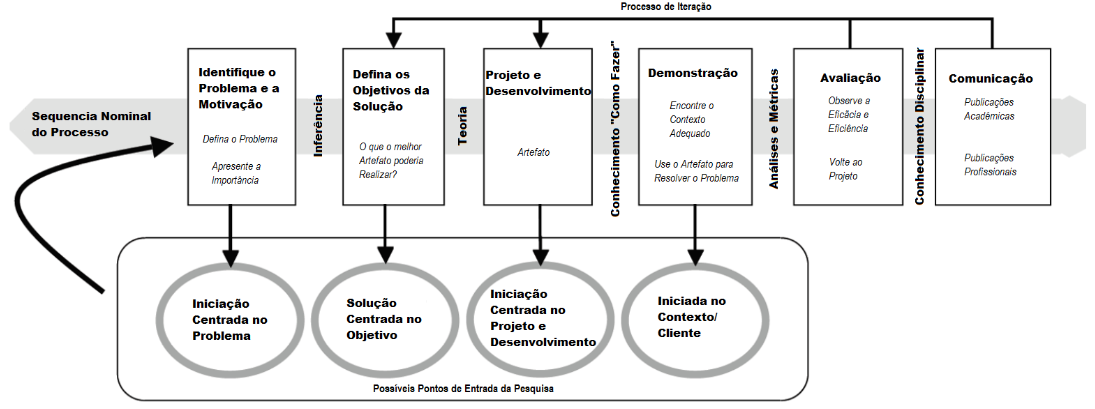
\includegraphics[scale=0.4]{Design-Science-Research03.png}
  \fonte{Adaptada de \textit{\citeauthor{peffers_dsr_2007}}}~\label{fig:processoDSR}
\end{figure}

% FAZER
% Pegar no de Marcelo, Falar mais sobre DSR e a parte dos artefatos e compartilhamento, Github e UnEB. Usar nota de rodapé para o link
% Para auxiliar no processo de gerenciamento e desenvolvimento dos artefatos, foram utilizadas outras duas ferramentas, trello e github...
% Escrever sobre as ferramentas
Também será utilizada análises quantitativas, ou seja, medidas estatísticas para mensurar e comparar os resultados obtidos.\\
Em suma, a pesquisa quantitativa só tem sentido quando há um problema muito bem definido e há informação e teoria a respeito do objeto de conhecimento, entendido aqui como o foco da pesquisa e/ou aquilo que se quer estudar. Esclarecendo mais, só se faz pesquisa de natureza quantitativa quando se conhece as qualidades e se tem controle do que se vai investigar~\cite{da_silva_pesquisa_2014}.

\section{Ambiente Experimental e Ciclo de Experimentos}
Esta seção descreve o ambiente experimental utilizado para o desenvolvimento do trabalho e a realização dos experimentos. É essencial compreender o contexto no qual os testes foram conduzidos, incluindo as especificações da máquina utilizada.

\begin{itemize}

  \item \textbf{Configurações do Ambiente:}
        O desenvolvimento do presente trabalho e a execução dos experimentos foram realizados em um sistema operacional Linux Ubuntu na versão 22.04.3 \gls{lts} x86\textunderscore64. As características fundamentais do computador são detalhadas abaixo:
        \begin{itemize}
          \item Kernel: 6.2.0{-}37-generic.
          \item \gls{cpu}: AMD Ryzen 9 7900 (24 núcleos) 3.700GHz
          \item Memória 32\gls{gigabyte}
        \end{itemize}

        Essa máquina está integrada ao ambiente do \gls{g2bc}, fornece do uma infraestrutura computacional robusta para proporcionar um ambiente robusto e eficiente para o desenvolvimento do código, bem como para a execução dos experimentos necessários.

  \item \textbf{Ciclo de Experimentos:}
        Os experimentos foram conduzidos em um ciclo iterativo para garantir a consistência e a validade dos resultados obtidos. Cada iteração envolveu a execução do código no ambiente descrito acima, seguida pela análise cuidadosa dos resultados e possíveis ajustes nos parâmetros experimentais.

        Este ciclo permitiu o aperfeiçoamento contínua da abordagem experimental, assegurando a confiabilidade e relevância dos resultados apresentados neste trabalho.

\end{itemize}
\section{Materiais e Métodos}
Nesta sessão, será apresentada as ferramentas utilizadas para a construção e desenvolvimento de todo o trabalho.

O Python é uma linguagem de programação de alto nível, interpretada, iterativa e de código aberto. Foi criada por Guido van Rossum e lançada em 1991 e é conhecida por ter uma sintaxe simples, tornando-a popular para o desenvolvimento de software, automação, análise de dados, aprendizado de máquina entre outras aplicações. A mesma apresenta suporte a vários paradigmas de programação, como a orientada a objetos, imperativa, procedural e funcional. Além disso, o Python é portátil, podendo ser executado em diversos sistemas operacionais como Linux, Mac e Windows~\cite{python-reference}.

Dessa forma, para a construção dos pipelines do projeto, utilizamos Python em conjunto com o Jupyter Notebook, o qual é uma aplicação de código aberto que permite criar documentos interativos que integram código, texto narrativo e visualizações. É uma ferramenta amplamente adotada por cientistas de dados, pesquisadores e desenvolvedores para explorar dados, prototipar código, documentar projetos e facilitar a colaboração. Além disso, ele oferece suporte a diversas linguagens de programação, incluindo Python~\cite{jupyter-notebook}.

O python possui uma gama de bibliotecas que facilitam a implementação de soluções complexas. A seguir serão apresentadas a bibliotecas utilizadas:

\begin{itemize}
  \item \textbf{Biopython}: Coleção de bibliotecas e ferramentas em Python, disponíveis gratuitamente para biologia molecular computacional. Ele fornece uma ampla gama de funcionalidades, desde a leitura e análise de arquivos de sequência biológica até a execução de algoritmos sofisticados de bioinformática. Desenvolvido e mantido pelo Projeto Biopython, que é uma associação internacional de desenvolvedores de ferramentas python~\cite{biopython}.
  \item \textbf{Selenium}: Biblioteca de código aberto que fornece uma interface programática para automatizar interações com navegadores da web. É amplamente utilizado por desenvolvedores e testadores de software para realizar testes automatizados, raspagem de dados na web e outras tarefas que envolvem interações com páginas da web. O Selenium para Python permite a automação de ações como clicar em botões, preencher formulários, navegar em sites e extrair informações da web, tornando-o uma ferramenta valiosa para desenvolvimento e automação de tarefas na web~\cite{selenium-python}.
\end{itemize}

% Lista de Tecnologias/Ferramentas utilizadas:
% Python 3 ok
% Selenium ok
% Biopython ok
% Shell (verificar necessidade)
% Jupyter Notebook ok
% Minimap2
% GoFasta
% virtualEnv

\section{Plano de Implementação}
Durante o desenvolvimento do projeto foi necessário dividi-lo em fases com base nas atividades que deveriam ser realizadas de forma a atender todos os passos descritos na seção~\ref{sec:metodologia}. As principais fases identificadas foram: Montagem e preparação do dataset a ser utilizado pelo modelo; Desenvolvimento completo do modelo, com todos as definições, implementações, testes e correções necessárias; e a análise comparativa que será realizada com um outro método existente e já tradicional. Esses pontos são apresentados de forma minuciosa a seguir.

\subsection{Montagem e Preparação do Dataset}
% FAZER
% Adicionar nota de rodapé com o link do repositório no Github
% Adicionar que o máximo de sequências baixadas por tipo foi de 10000 (dez mil). Limite máximo de sequências por vez aplicado pela própria plataforma. Sendo selecionadas as primeiras 10k
Para realizar o treinamento do modelo a ser construído, eram necessárias sequências únicas e alinhadas do gene Spike. Em vista disso, é importante salientar que o site \gls{bvbrc} disponibiliza sequências genômicas, e sendo assim, foi preciso construir um pipeline para, após o download delas, transforma-las para a criação de um dataset com aquelas que atendessem os requisitos esperados.

Inicialmente, foi realizada uma analise do \gls{bvbrc}, para entender a sua estrutura e verificar também se era possível realizar o \textit{download} de todas as sequências essenciais de forma manual. Em seguida, foi verificado que o site possuía uma área de seleção de filtros, e que só era possível selecionar dez mil sequências por vez. Além disso, foi definido que só seriam selecionadas sequências completas no campo \textit{Genome Status} e no campo \textit{Lineage}, onde é possível filtrar as sequências pelo seu tipo \textit{Pango} e também verificar a quantidade, só as que tivessem mais de 50 seriam selecionados.

Após a análise, foi constatado que realizar o download manualmente era infactível, e que seria preciso automatizar esse processo de iteração com a página, como vistos na Figura~\ref{fig:pipelineBvbrc}. Isto posto, foi realizado uma sequência de passos conhecidos como \textit{Web Scrapping} utilizado o Python juntamente com o Selenium, apresentados em seguida:

\begin{figure}[htb]
  \centering
  \caption{Pipeline de Download das Sequências Genômicas.}
  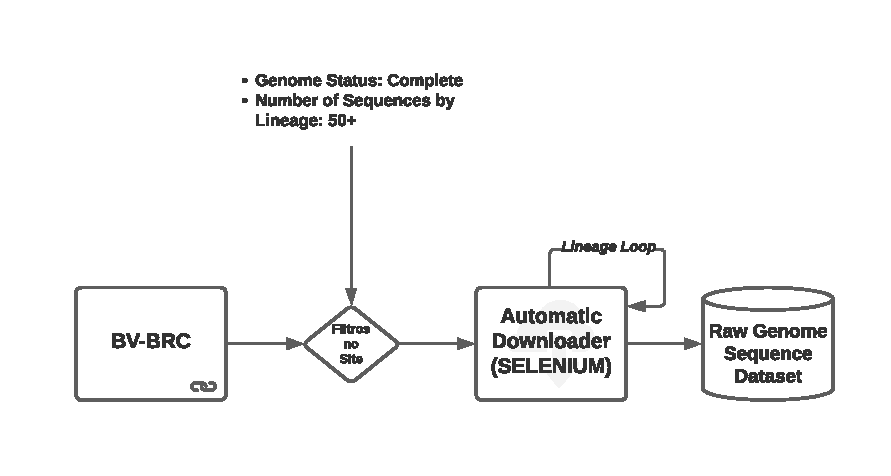
\includegraphics[scale=0.6]{pipelines/bvbrc.pdf}
  \fonte{O Autor}~\label{fig:pipelineBvbrc}
\end{figure}

\begin{enumerate}
  \item Criar uma lista com todas as linhagens disponíveis e a quantidade de sequências de cada.
  \item Desenvolver script Python para remover as linhagens com menos de 50 sequências da lista.
  \item Desenvolver script Python para gerar uma url personalizada do \gls{bvbrc}, já com os filtros, para cada linhagem.
  \item Desenvolver script Python juntamente com o Selenium para abrir as urls de forma automática e realizar o download das sequências.
\end{enumerate}

Ao final do processo de montagem do dataset, realizado no dia 02 junho de 2023, com sequências genômicas completas, foi gerado um diretório raiz (dataset), e dentro desse, um diretório para cada linhagem (\textit{Lineage} L¹, \textit{Lineage} L², \dots, \textit{Lineage} $L^{n}$), contendo um arquivo nomeado \textnormal{BVBRC\_genome\_sequence.fasta}, como apresentado na figura~\ref{fig:datasetGenomas}.

\begin{figure}[htb]
  \centering
  \caption{Dataset de sequências genômicas.}
  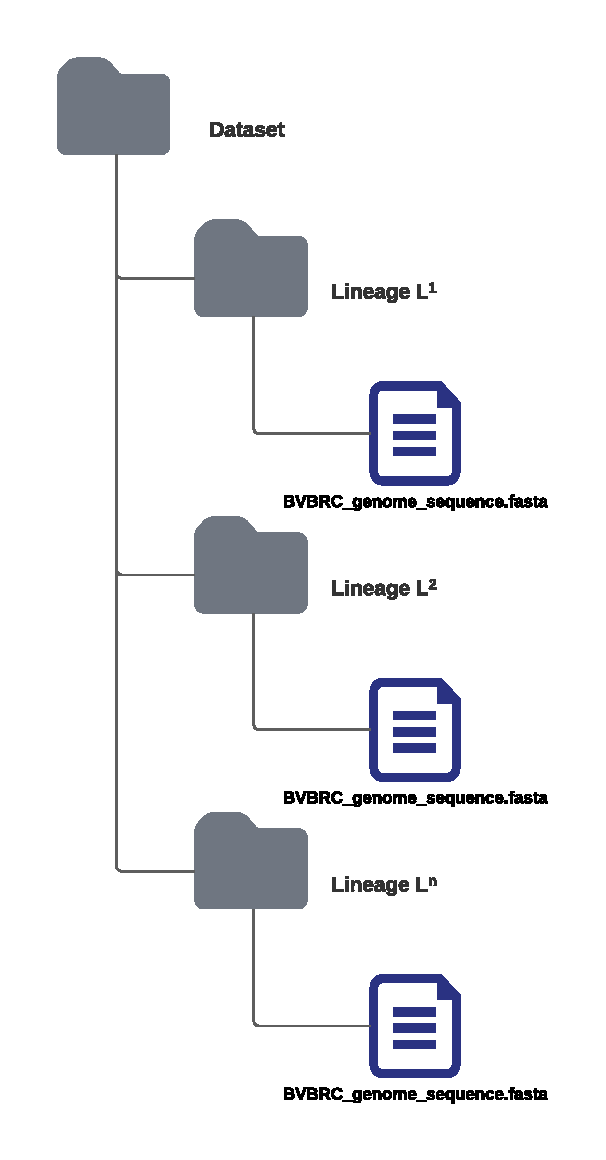
\includegraphics[scale=0.5]{figuras/dataset_principal.pdf}
  \fonte{O Autor}~\label{fig:datasetGenomas}
\end{figure}

Ao finalizar o processo de download, o \textit{dataset} completo ficou com as seguintes informações apresentadas na tabela~\ref{tab:datasetGenomas}.

\begin{table}[htb]
  \caption{Informações do dataset de sequências genômicas.}
  \begin{center}
    \begin{tabular}{c|c}
      \hline
      Campo                              & Valor     \\
      \hline
      Quantidade de Linhagens            & 1086      \\
      Quantidade de Sequências Genômicas & 1.494.650 \\
      Tamanho em \gls{gigabyte}          & 47.5      \\
      \hline
    \end{tabular}
  \end{center}
  \fonte{O Autor}\label{tab:datasetGenomas}
\end{table}

A seguir, era necessário construir um dataset de sequências do gene Spike a partir do existente. Para isso, com o objetivo de diminuir o tempo de execução dos pipelines durante o desenvolvimento, foi construído também, um dataset de testes, exposto na tabela~\ref{tab:datasetGenomasTeste}, que serviriam como base para execução das atividades, e após as verificações, seria realizado o processo com o dataset completo. No dataset de testes, foram escolhidas 5 (cinco) linhagens que são amplamente conhecidas (alpha, beta, gamma, delta e omicron), o que tornaria mais preciso o processo de validação futuramente.

\begin{table}[htb]
  \caption{Informações do dataset de teste de sequências genômicas.}
  \begin{center}
    \begin{tabular}{c|c|c|c}
      \hline
      Pango     & \gls{who} & Quantidade de Sequências & Tamanho em \gls{megabyte} \\
      \hline
      B.1.1.7   & Alpha     & 9982                     & 307                       \\
      B.1.351   & Beta      & 5256                     & 160.6                     \\
      P.1       & Gamma     & 10000                    & 305.9                     \\
      B.1.617.2 & Delta     & 9996                     & 305.3                     \\
      B.1.1.529 & Omicron   & 3694                     & 112.7                     \\
      \hline
      Total     &           & 38928                    & 1191,5                    \\
      \hline
    \end{tabular}
  \end{center}
  \fonte{O Autor}\label{tab:datasetGenomasTeste}
\end{table}

Depois, foi verificado a existência de sequências genômicas idênticas, melhor dizendo, sequências com exatamente a mesma quantidade e ordem dos nucleotídeos. Por essa razão, foi necessário desenvolver um pipeline que filtrasse as sequências repetidas, e mantivesse apenas uma, como exibido na figura~\ref{fig:pipelineGenomicasDuplicadas}, gerando assim um novo dataset de sequências genômicas únicas.

\begin{figure}[htb]
  \centering
  \caption{Pipeline de Filtragem de Sequências Genômicas Duplicadas.}
  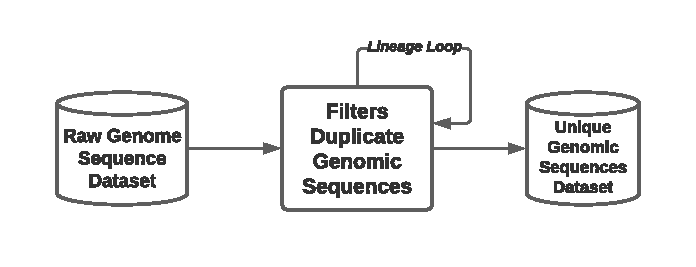
\includegraphics[scale=0.6]{pipelines/filtrando_genomas_duplicados.pdf}
  \fonte{O Autor}~\label{fig:pipelineGenomicasDuplicadas}
\end{figure}

Com o dataset de sequências únicas montado, foi decidido os passos a seguir, que seriam executados com o papel de atingir o objetivo de obter o dataset de sequências gênicas únicas e alinhadas. Primeiro, como visto na figura~\ref{fig:pipelinesDescontinuados}, foi realizado o processo de extração do gene Spike, utilizando uma sequência de referência do gene obtida do dataset da \gls{ncbi}\footnote{Url para download: \url{https://www.ncbi.nlm.nih.gov/nuccore/NC_045512.2?report=genbank&from=21563&to=25384}}, juntamente com o software Blast, para encontrar e extrair o gene Spike de cada uma das sequências genômicas de todo o dataset. Após isso, com o dataset de sequências gênicas já montado, era necessário realizar o processo de alinhamento. Foram verificada duas formas de realizar esse procedimento utilizando o software Clustalo Omega: passando uma sequência por vez (\textit{sequence by sequence}) com a sequência do Spike de referência; e outra passando todas as sequências com a referência (\textit{multiple sequence}). Entretanto, mesmo com o dataset de teste, que possuía um tamanho muito inferior ao principal, o processo de alinhamento apresentou uma demora excessiva (até 2 dias) para finalizar. Em decorrência disso, o processo foi descontinuado, e um novo foi repensado e reconstruído e será apresentado a seguir.

\begin{figure}[htb]
  \centering
  \caption{Pipelines descontinuado.}
  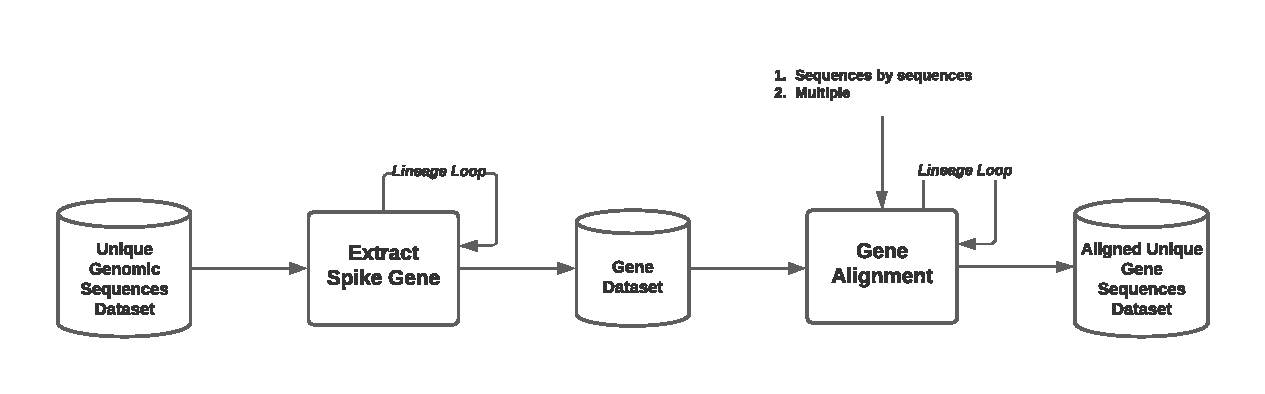
\includegraphics[scale=0.7]{pipelines/pipelines_descontinuado.pdf}
  \fonte{O Autor}~\label{fig:pipelinesDescontinuados}
\end{figure}

% FAZER
% Como escrever essa parte: Após análise; Após orientação do coorientador...
% Reescrever a lista abaixo de forma descritiva
% Substituir onde estiver citando 'modelo desenvolvido' pelo nome AGUA
Após um processo de análise, o desenvolvimento continuou a partir das sequências genômicas únicas, foi feito seguindo os quatro (4) passos apresentados a seguir:

\begin{enumerate}
  \item \textbf{Alinhamento das sequências genômicas:} A primeira etapa, como apresentado na figura~\ref{fig:alinhamentoGenomas}, consistiu em alinhar as sequências genômicas únicas já disponíveis, utilizando a ferramenta de alinhamento Minimap2, a qual é um recurso eficiente para mapear sequências em um genoma de referência~\cite{minimap2_li_2018}. E esse processo permitiu a identificação de regiões específicas relacionadas ao gene spike.
        \begin{figure}[htb]
          \centering
          \caption{Pipeline de Alinhamento de Sequências Genômicas Duplicadas.}
          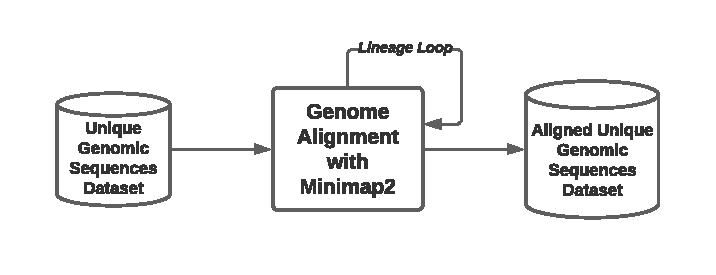
\includegraphics[scale=0.6]{pipelines/alinhamento_genomas_minimap2.pdf}
          \fonte{O Autor}~\label{fig:alinhamentoGenomas}
        \end{figure}
  \item \textbf{Extração do Gene Spike com Uso de Isca:} Após o alinhamento, as sequências de referência do gene spike foram usadas como ``iscas'' para identificar e extrair aquelas correspondentes nas sequências genômicas alinhadas, como visto na figura~\ref{fig:extracaoSpike}. O gene spike é de importância crítica, pois desempenha um papel fundamental na interação do vírus com as células hospedeiras. Ou seja, a utilização de iscas garantiu que uma extração correta do genoma completo.
        \begin{figure}[htb]
          \centering
          \caption{Pipeline de Extração do Gene Spike das Sequências Genômicas Alinhadas.}
          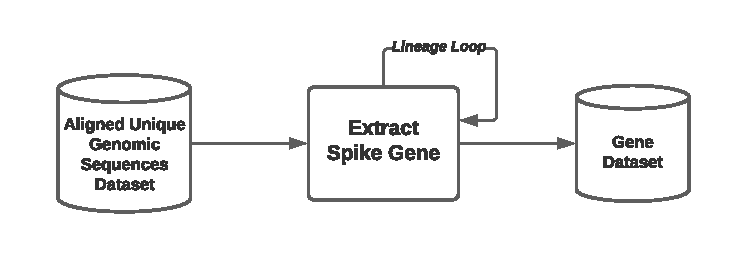
\includegraphics[scale=0.6]{pipelines/extraindo_gene_spike.pdf}
          \fonte{O Autor}~\label{fig:extracaoSpike}
        \end{figure}
  \item \textbf{Filtragem de Sequências Genicas Duplicadas:} Uma das preocupações na criação do dataset foi a presença de sequências duplicadas, que podem enviesar os resultados da análise. Portanto, as que estavam repetidas foram identificadas e removidas do conjunto de dados. Esse processo garantiu que cada sequência fosse única, evitando redundâncias.
        \begin{figure}[htb]
          \centering
          \caption{Pipeline de Filtragem de Sequências Genicas Duplicadas.}
          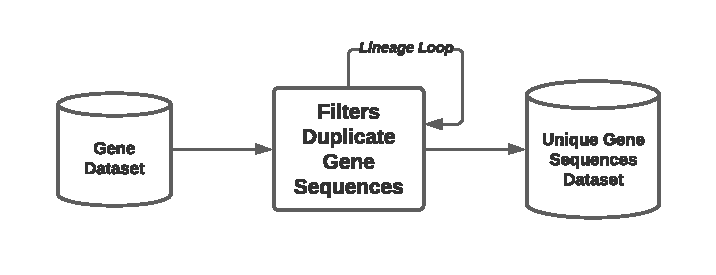
\includegraphics[scale=0.6]{pipelines/filtrando_spikes_duplicados.pdf}
          \fonte{O Autor}~\label{fig:spikeDuplicados}
        \end{figure}
  \item \textbf{Filtragem de Sequências de Má Qualidade:} Para garantir a qualidade do dataset, as sequências genômicas que continham características indesejáveis foram filtradas. Isso incluiu a remoção das que continham mais de 30 bases nitrogenadas (N) consecutivas e aquelas que não correspondiam ao tamanho esperado das sequências de referência do gene spike como visto na imagem~\ref{fig:spikesRuins}. Essa purificação ajudou a garantir que as sequências incluídas no dataset fossem de alta qualidade e relevantes para a análise subsequente.
        % FAZER: Corrigir parte que fala dos Ns
        \begin{figure}[htb]
          \centering
          \caption{Pipeline de Filtragem de Sequências Genicas de Má Qualidade.}
          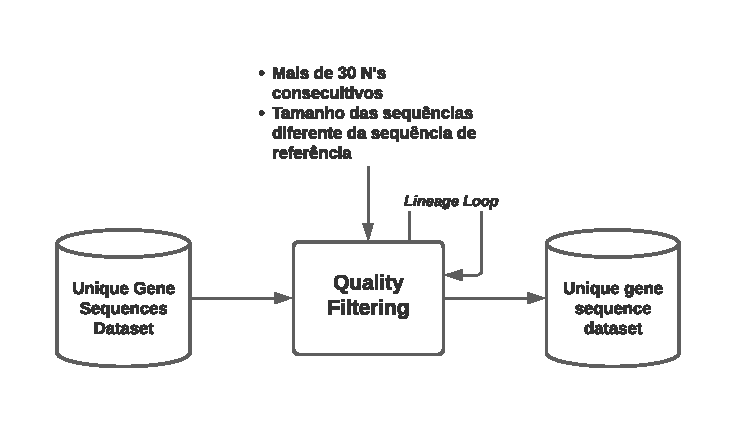
\includegraphics[scale=0.6]{pipelines/filtrando_spikes_ruins.pdf}
          \fonte{O Autor}~\label{fig:spikesRuins}
        \end{figure}
\end{enumerate}

Ao final do processo, foi gerado um \textit{dataset} de alta qualidade, contendo sequências gênicas únicas para as variantes alpha, beta, gamma, delta, e omicron. E ele será a base para a análise de genes virais com base no uso de códons e a aplicação de técnicas de classificação não supervisionada.

A partir deste dataset, foi elaborado 2 (dois) arquivos, conforme a figura~\ref{fig:inputAgua} apresenta, que serviria de entrada, tanto para o modelo desenvolvido como para a geração de árvores filogenéticas utilizando o modelo convencional, a fim de se realizar análises futuras. Um arquivo compreendia a mescla de sequências genicas de cada uma das linhagem, e outro anotações que serviria como base no treinamento, contendo o cabeçalho da sequência, na mesma ordem em que estava no arquivo mesclado, juntamente com a linhagem da sequência.

\begin{figure}[htb]
  \centering
  \caption{Arquivos de Entrada do AGUA.}
  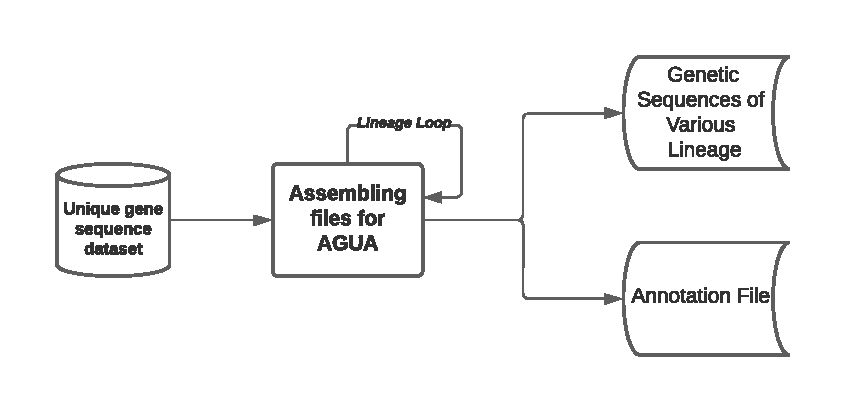
\includegraphics[scale=0.7]{pipelines/input_agua.pdf}
  \fonte{O Autor}~\label{fig:inputAgua}
\end{figure}

\subsection{AGUA}
O modelo proposto foi designado como \gls{agua}. A subsequente seção discorrerá detalhadamente sobre os procedimentos metodológicos que foram seguidos para a formulação e concepção do referido modelo. Este processo envolveu uma série de etapas meticulosas e estrategicamente delineadas, as quais serão elucidadas a seguir, contribuindo para uma compreensão aprofundada de sua elaboração.

% FAZER
% Escrever uma descrição melhor do desenvolvimento do modelo
\begin{itemize}
  \item Levantamento dos requisitos.
  \item Definição da arquitetura e abordagem do modelo de classificação baseado em códons.
  \item Implementação do modelo utilizando bibliotecas adequadas.
        % \item Desenvolver algoritmo para traduzir as sequências de \gls{dna} em sequências de códons.
  \item Treinamento do modelo.
  \item Avaliação de desempenho utilizando métricas apropriadas.
        % \item \item Avaliar o desempenho do modelo utilizando métricas apropriadas, como acurácia, precisão e recall.
  \item Identificação de problemas e realização de ajustes.
        % \item Identificar possíveis problemas de overfitting ou underfitting e realizar ajustes no modelo, como ajuste de hiperparâmetros ou utilização de técnicas de regularização.
\end{itemize}

Prosseguindo com a sequência metodológica delineada anteriormente, será detalhada de maneira prática a implementação do \gls{agua}. Este segmento apresentará o resultado tangível desse processo, traduzido em código. As implementações e estruturações técnicas discutidas a seguir representam a concretização do modelo, oferecendo uma visão aprofundada de suas características fundamentais e contribuições efetivas no âmbito abordado. Para facilitar revisões e colaborações, o código-fonte encontra-se disponibilizado na plataforma de hospedagem GitHub, no repositório do \gls{g2bc}~\footnote{Url do repositório: \url{https://github.com/G2BC/agua}}.

O processo inicia-se com a leitura das sequências do gene spike de um arquivo no formato {FASTA}. Após isso, as sequências são verificadas quanto ao seu tamanho, assegurando que sejam múltiplos de 3, um requisito fundamental para a correta representação de códons. Posteriormente, ocorre a conversão das sequências de nucleotídeos em códigos numéricos, representando códons, sendo realizado através do algoritmo \gls{cbuc}, desenvolvido pelos graduandos Diego dos Santos Fonseca, Cândido Luiz do Nascimento Júnior e o {Prof.} Drº. Diego Gervasio Frías Suárez~\cite{identificacao_cbuc_diego_2021,spike_cbuc_candido_2021}.

As sequências de códons resultantes passam por uma filtragem, removendo sequências que contenham códons de parada no final. A matriz de sequência de códons é então processada, convertida para um array \textit{numpy}~\cite{numpy_van_2011}, e a contagem dos códons distintos por coluna é realizada. Calcula-se a variabilidade de códons em cada coluna, selecionando aquelas com variabilidade maior que 1, indicando a presença de mais de um tipo de códon.

Para cada sequência, uma lista de ID's é gerada contendo os códons nas colunas selecionadas, e após isso são convertidos em \textit{strings}. A geração de ID's para as classes primárias das sequências segue a identificação e seleção de classes primárias únicas, associadas a números. Um \textit{DataFrame} é criado usando a biblioteca Pandas para organizar as informações do \gls{gvf}.

A aplicação do algoritmo de \textit{clustering} Clope otimiza a distribuição de transações em clusters para maximizar uma função objetivo\cite{Clope_yang_2002}. E, apesar do agrupamento com o Clope ser não supervisionado, o código utiliza-se das anotações, para otimizar a escolha do seu único parâmetro ajustável, chamado de repulsão (\textit(repulsion)), buscando a melhor resolução de agrupamento para um conjunto de dados de sequências genéticas. Este processo visa encontrar configurações que produzam agrupamentos com alta resolução, onde as sequências pertencentes ao mesmo cluster sejam homogêneas em termos de genótipo, em comparação com os rótulos reais fornecidos no \textit{ground truth} de anotação.

O código, então, realiza a leitura de um arquivo de anotações e otimiza a escolha do valor de repulsão. A matriz de confusão entre as espécies (anotações) e os clusters é gerada, indicando como as espécies reais foram agrupadas nos clusters encontrados pelo algoritmo Clope. A identificação de clusters contendo múltiplas espécies é realizada, seguida pelo cálculo de uma matriz de distâncias entre pares de classes primárias.

Por fim, o código utiliza a biblioteca SciPy para realizar a ligação hierárquica com diferentes métodos de ligação, gerando árvores filogenéticas que são plotadas a partir dos resultados da análise. Ao final do processo, a biblioteca Dill é utilizada para serializar o objeto e gravar o modelo~\cite{dill}.

Ao fim do processo o \gls{agua} tem como suas saídas: uma matriz de distâncias, que pode ser utilizada para construir dendrogramas e o modelo treinado com as sequências.

\subsection{Análise comparativa entre o método proposto (AGUA) e outro método existente}
Nesta seção, apresentamos uma análise comparativa detalhada entre o método proposto e um tradicional amplamente utilizado. O objetivo é avaliar o desempenho e a eficácia do nosso método em relação a uma abordagem estabelecida. Para esse fim, realizamos a investigação em um conjunto de dados comum apresentado na figura~\ref{tab:datasetGenomasTeste}. O método tradicional selecionado para comparação é o utilizando no \textit{software} IQ-TREE, que é um estimador de máxima verossimilhança de alta performance, frequentemente empregado na filogenia molecular~\cite{iqtree2_minh_2020}.

A escolha do IQ-TREE como método tradicional se baseia em sua prevalência na comunidade científica e sua eficácia comprovada em construir árvores filogenéticas a partir de dados de sequenciamento. A avaliação comparativa entre o método proposto e o IQ-TREE nos permitirá avaliar a capacidade do nosso modelo em produzir resultados relevantes e precisos em comparação com uma abordagem estabelecida.

Considerando o propósito de realizar uma comparação entre os métodos, procedeu-se à análise do tempo de execução de cada um deles, variando tanto o número de linhagens quanto a quantidade de sequências. No que diz respeito ao número de linhagens, foram consideradas 2 (Alpha e Beta) para o conjunto L1, 3 (Alpha, Beta e Gamma) para o conjunto L2, 4 (Alpha, Beta, Gamma e Delta) para o conjunto L3 e 5 (Alpha, Beta, Gamma, Delta e Omicron) para o conjunto L4, em cada conjunto de dados. Em relação à quantidade de sequências, foram contemplados 100 (T100), 300 (T300), 500 (T500) e 700 (T700) sequências para cada categoria.
A tabela~\ref{tab:quantidadeSequenciasTeste} apresenta o total de sequências em cada um dos testes que foram montados.
Dessa forma, estabeleceram-se cenários variados para avaliação dos métodos, considerando diferentes combinações de linhagens e quantidades de sequências.

\begin{table}[htb]
  \caption{Quantidade de sequências por treinamento utilizados para testes de performance nos dois modelos.}
  \begin{center}
    \begin{tabular}{c|c|c|c|c}
      \hline
      Linhagens & T100 & T300 & T500 & T700 \\
      \hline
      L1        & 200  & 600  & 1000 & 1400 \\
      L2        & 300  & 900  & 1500 & 2100 \\
      L3        & 400  & 1200 & 2000 & 2800 \\
      L4        & 500  & 1500 & 2500 & 3500 \\
      \hline
    \end{tabular}
  \end{center}
  \fonte{O Autor}\label{tab:quantidadeSequenciasTeste}
\end{table}

A abordagem metodológica consiste em utilizar o mesmo conjunto de sequências do gene spike, que alimentou o \gls{agua} para a construção de árvores filogenéticas usando o IQ-TREE como apresentado na figura~\ref{fig:inputAguaIqtree}. Comparamos, então, o tempo de processamento em ambos os casos. Essa análise comparativa nos permitirá determinar se o método proposto representa uma melhoria significativa em relação à abordagem tradicional, contribuindo assim para o avanço no campo da filogenia molecular.
\begin{figure}[htb]
  \centering
  \caption{Arquivos de entrada do AGUA e do IQ-TREE.}
  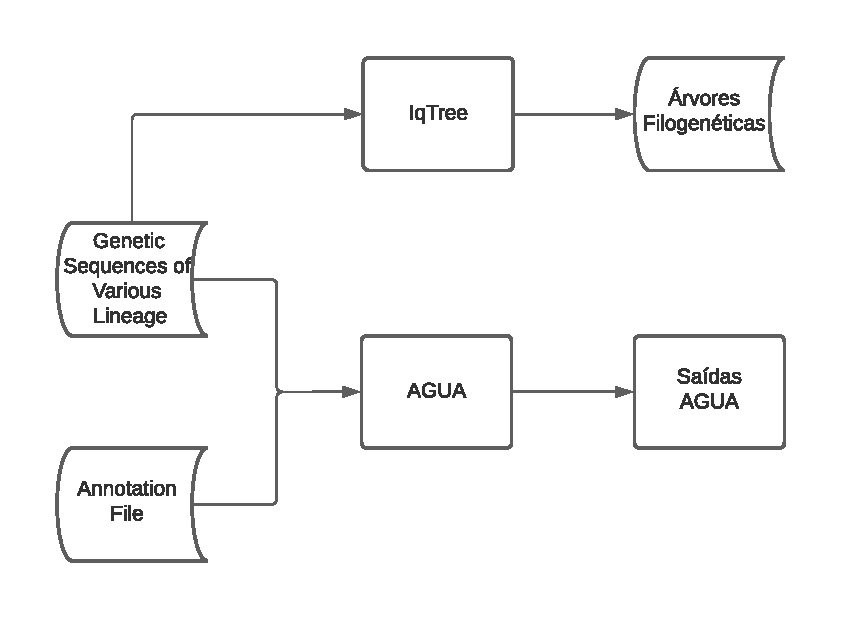
\includegraphics[scale=0.7]{pipelines/agua_iqtree2.pdf}
  \fonte{O Autor}~\label{fig:inputAguaIqtree}
\end{figure}

Os testes foram executados conforme os parâmetros apresentados na tabela~\ref{tab:quantidadeSequenciasTeste}. Os tempos de processamento para o \gls{agua} são apresentados na tabela~\ref{tab:tempoProcessamentoAgua} e os tempos do IQ-TREE na tabela~\ref{tab:tempoProcessamentoIqtree}. Além disso foi gerado árvores nos dois modelos, a do \gls{agua} é apresentada no Anexo~\ref{an:arvore_agua}, já a árvore filogenética gerada pelo IQ-TREE é apresentada no Anexo~\ref{an:arvore_iqtree}, a mesma foi plotada utilizando o \textit{software} Figtree. Destaca-se que, devido à limitação de tempo, está pesquisa não empreenderá qualquer avaliação das árvores geradas.

\begin{table}[htb]
  \caption{Tempo de processamento, em segundos, das sequências gênicas com o AGUA.}
  \begin{center}
    \begin{tabular}{c|c|c|c|c}
      \hline
      Linhagens & T100   & T300    & T500    & T700     \\
      \hline
      L1        & 63.94  & 518.85  & 1309.27 & 2478.68  \\
      L2        & 160.76 & 1242.55 & 2992.54 & 5589.52  \\
      L3        & 298.78 & 2302.29 & 5804.33 & 9878.99  \\
      L4        & 438.31 & 3696.73 & 8910.84 & 15877.98 \\
      \hline
    \end{tabular}
  \end{center}
  \fonte{O Autor}\label{tab:tempoProcessamentoAgua}
\end{table}

\begin{table}[htb]
  \caption{Tempo de processamento, em segundos, das sequências gênicas com o IQ-TREE.}
  \begin{center}
    \begin{tabular}{c|c|c|c|c}
      \hline
      Linhagens & T100  & T300   & T500   & T700   \\
      \hline
      L1        & 62.18 & 93.40  & 105.20 & 151.04 \\
      L2        & 76.38 & 95.33  & 121.06 & 177.27 \\
      L3        & 75.41 & 111.26 & 324.65 & 281.13 \\
      L4        & 76.69 & 131.25 & 210.89 & 393.44 \\
      \hline
    \end{tabular}
  \end{center}
  \fonte{O Autor}\label{tab:tempoProcessamentoIqtree}
\end{table}

% FAZER Verificar essa parte
Embora os resultados de tempo de processamento indiquem que o método alternativo apresentou um desempenho mais rápido em comparação com o \gls{agua} em todos os cenários avaliados, é crucial ressaltar que a eficiência temporal não é o único critério para avaliar a robustez de um método. O \gls{agua}, apesar de requerer mais tempo computacional, oferece uma abordagem inovadora para a classificação de linhagens, incorporando aprendizado automático que pode melhorar significativamente a precisão da classificação.

É fundamental destacar que a escolha entre métodos deve levar em consideração não apenas a rapidez da execução, mas também a capacidade de adaptação a diferentes contextos e a qualidade das análises produzidas. O método proposto, \gls{agua}, prioriza a aprendizagem automática e, portanto, oferece uma solução mais robusta em termos de capacidade de classificação.

A rápida execução do método alternativo pode ser atribuída à sua natureza não supervisionada e pré-determinada, o que, embora eficiente em termos de tempo, limita sua adaptabilidade a diferentes conjuntos de dados. O \gls{agua}, ao empregar aprendizado automático, apresenta maior flexibilidade para ajustar-se a variações nos dados, resultando em classificações mais refinadas e adaptadas.

Em última análise, o \gls{agua} busca proporcionar não apenas uma alternativa eficiente em termos de tempo, mas uma abordagem mais completa e contextualizada para a classificação de linhagens. Ao integrar aprendizado automático, o \gls{agua} não só automatiza o processo, mas também aprimora a qualidade das análises, oferecendo uma contribuição valiosa para a compreensão da diversidade genética.

